\documentclass{amsart}
\usepackage{graphicx}
\graphicspath{{./}}
\usepackage{hyperref}
\usepackage{csvsimple}
\usepackage{longtable}
\usepackage{lscape}
\usepackage{epigraph}
\title{History of Exact Distributions in Science and Statistics}
\author{Zulfikar Moinuddin Ahmed}
\date{\today}
\begin{document}
\maketitle

\section{A Celebration of Barndorff-Nielsen Distribution of 1976}

I love history of ideas and discoveries and inventions, because it inspires me forward, and fills me with joy and optimism at the progress of my Beloved People the Human Race.  I would like to celebrate O. Barndorff-Nielsen's Discovery of Generalised Hyperbolic Distributions in 1976 as a singular event in the history of Science of the Human Race because these are the most important probability distributions in Nature.  It was I, Zulfikar Moinuddin Ahmed, who assessed and understood their full importance for the first time, but the great genius of Barndorff-Nielsen that led unerringly to the heart of Nature must be celebrated because nothing that the world had known till 1976 could have predicted such a monumental coup.  He had found precise mathematical formulae for the secret laws of Noise in Nature.  He could be akin to a Mage from some Fantasy Novel with Arcane Runes and esoteric Mathematical Formulae that reveal Nature's exact law for Noise.  The Normal Gaussian distribution is mere toy by comparison.  And I would know.  I singlehandedly provided the final law of macroscopic physics some years ago, and eviscerated the fake law of gravity and can assure human race that this universe does not have any mass-based laws at all.

He came 276 years later than James Bernoulli.  And this is interesting to me.  

\section{O. Barndorff-Nielsen is A Sophisticated Probability Theorist But His Discovery is Uncanny}

I have been doing mathematical Finance since 1995.  There are many interesting sophisticated ideas from stochastic process theory that are applied in Finance; to my credit is one of the best long memory stochastic volatility models in the world.  It's not enough to know sophisticated probability theory to actually have any success with inscrutible secrets of Nature.  Barndorff-Nielsen's success is so extraordinary that I am ready to believe that his soul could be a Dragon even, which would be quite alarming.  

Now I am an Archangel, I was firmly involved in the Dragon Wars about two billion years ago, and let me assure you that you should all be alarmed if Dragon Souls are born as humans these days.  Dragons totally annihilated each other across entire Galaxies as hunger for Magic and Power consumed them.  I don't want Human Race to be wiped out by Dragon Souls suddenly finding Earth as their base for Universal Conquest or whatever it is that gets Dragons excited.  Whew!

\section{Binomial Distribution of Jacob Bernoulli 1700}

James Bernoulli discovered the binomial law in 1700.

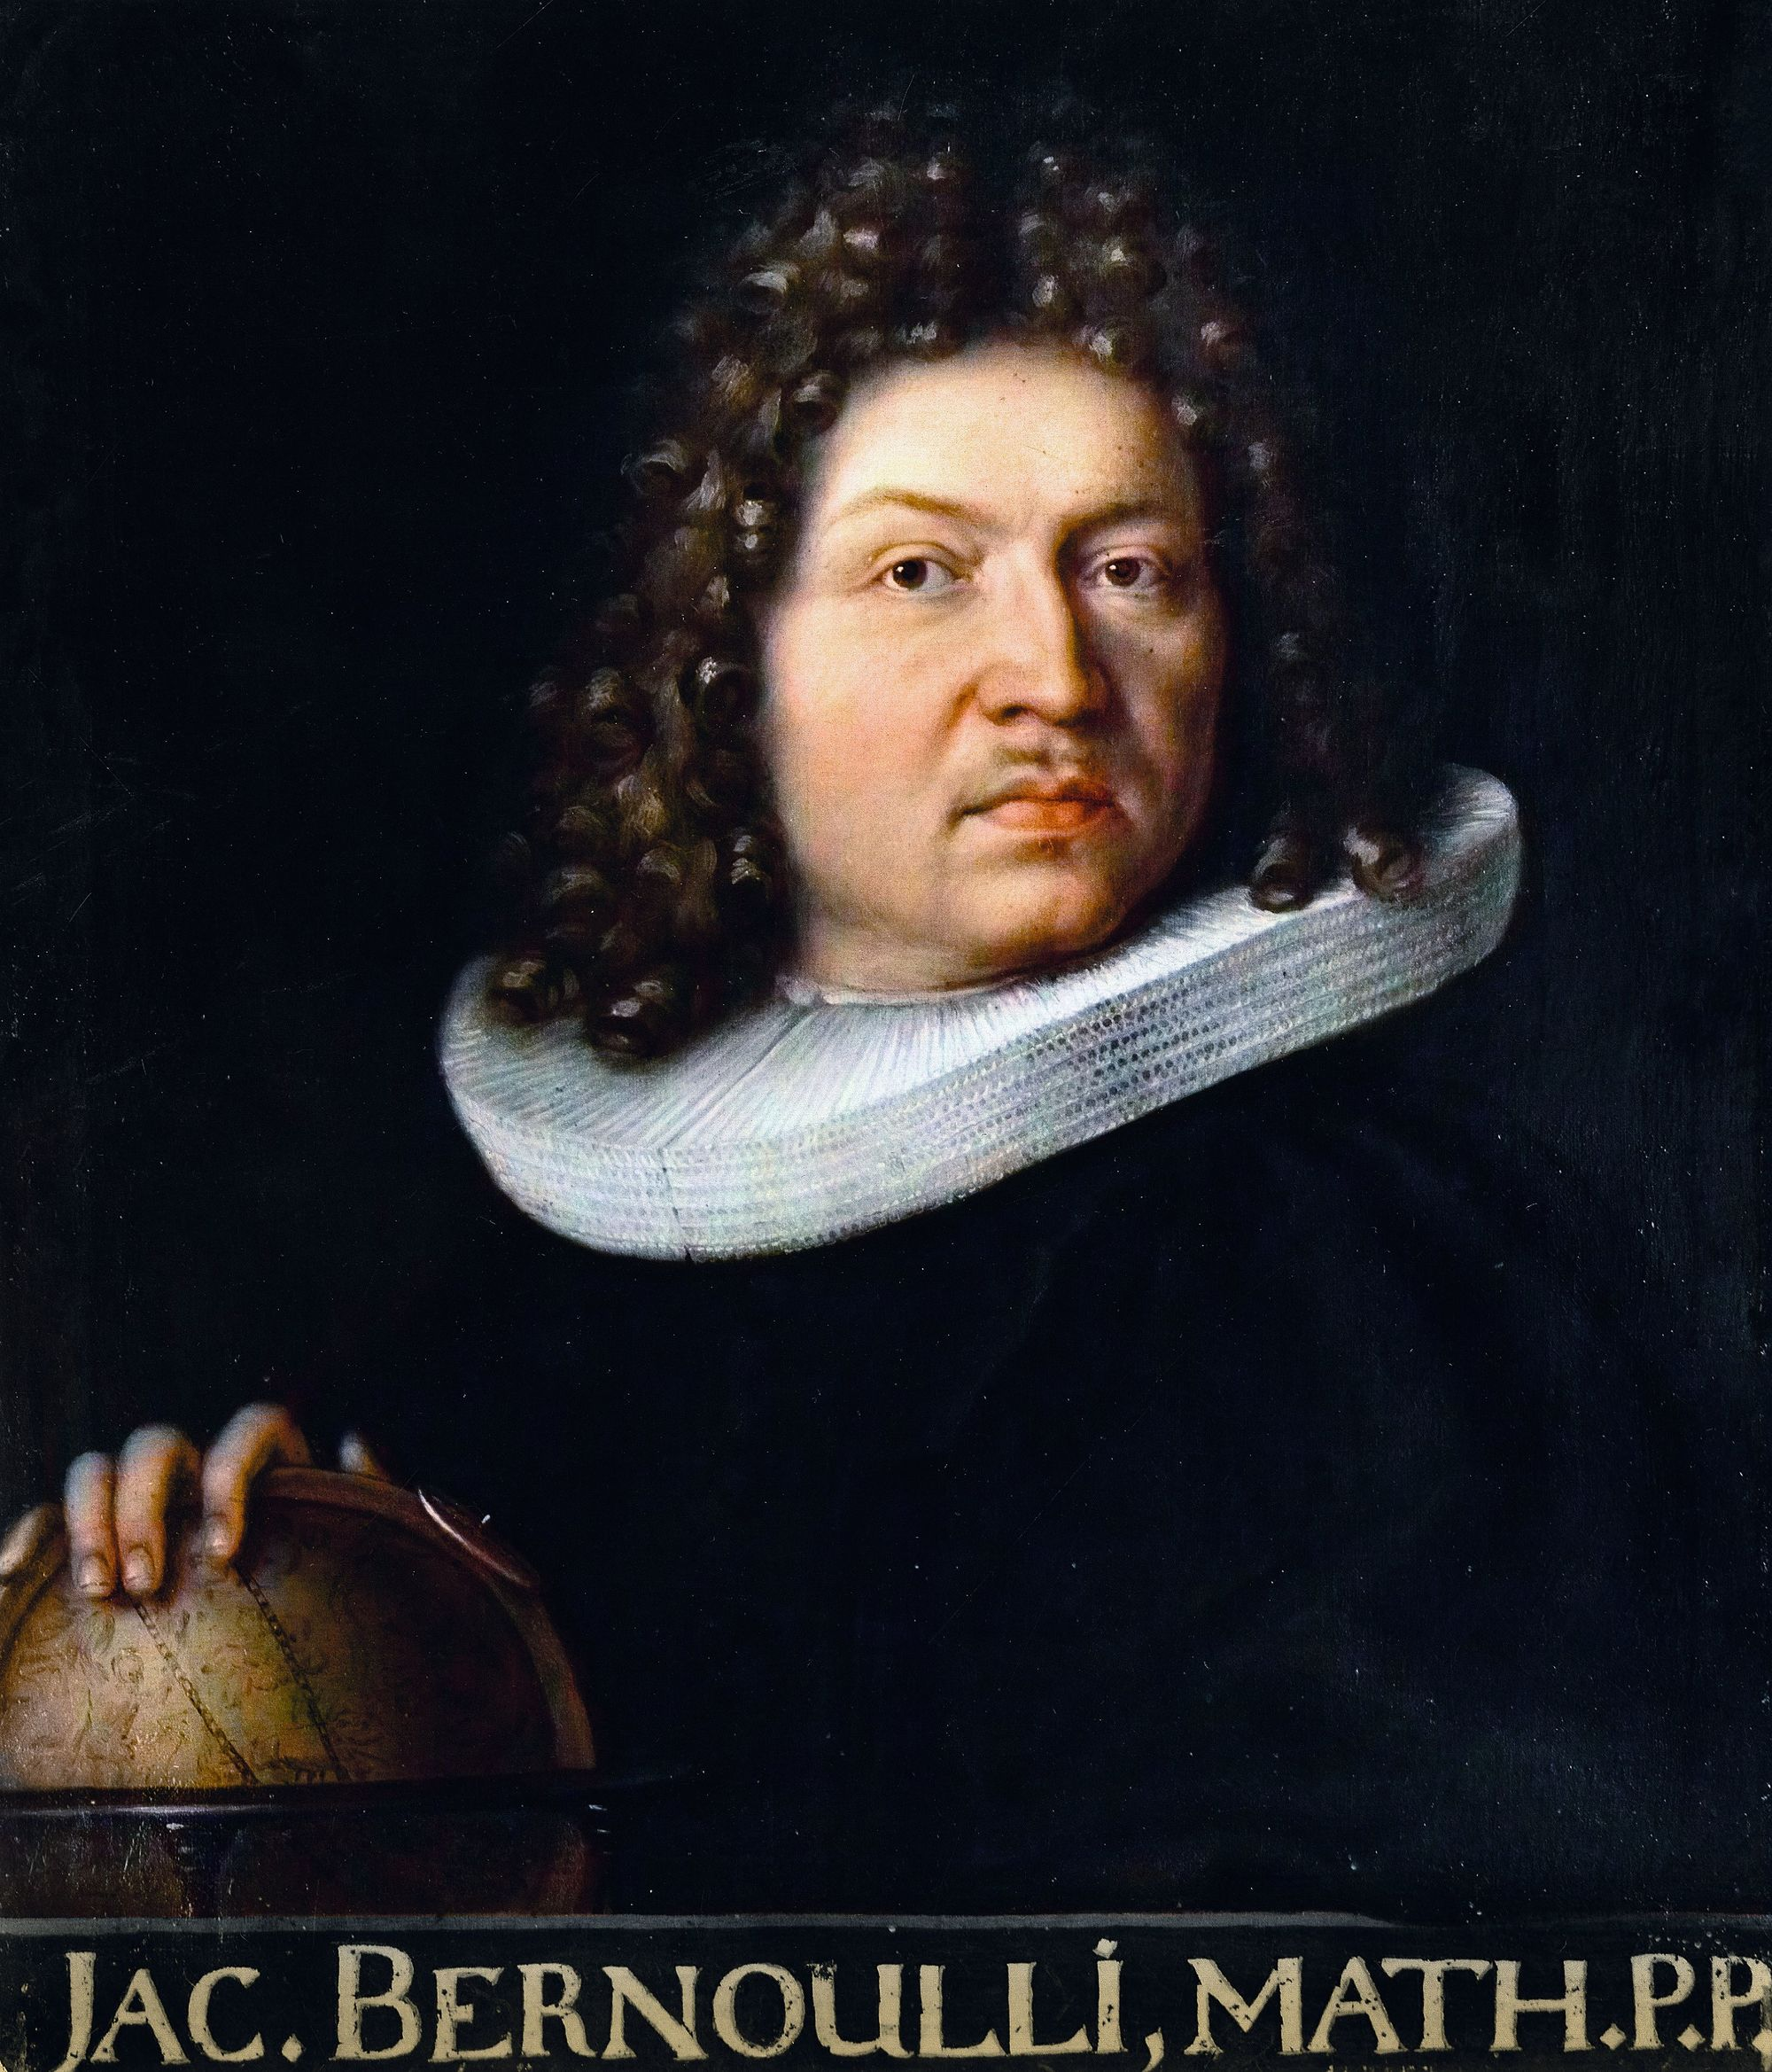
\includegraphics[scale=0.1]{bernoulli.jpg}

Today this is routine material.  Frequency distribution of ratios of heads and tails converge to their theoretical fractions is the Law of Large Numbers.  I won't go too much into this because today most high school students are quite able to appreciate the binomial coefficients and Pascal's triangle and such.

\section{Simeon Denis Poisson}

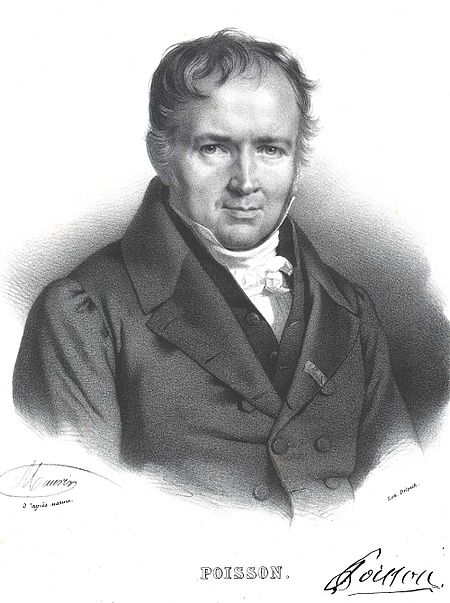
\includegraphics[scale=0.6]{poisson.jpg}

Poisson is responsible for the random variables on $\mathbf{N}$ given by 
\[
P(X = k ) = \frac{\lambda^k}{k!} e^{-\lambda}
\]
This is the Poisson distribution.  The continuous version is the exponential distribution.  It was my own discovery that in moral values, human beings have exponential distribution away from "Good".  Simeon-Denis Poisson was not doing something particularly of purely mathematical interest.  I hate the phrasing of 'applied mathematics'.  I am a pure devotee of Nature and consider devotion to Nature to be a separate matter than 'applied mathematics' because there is a different evolution of the Soul involved.  I am not actually doing 'applied mathematics'.  I truly despise this denigrating terminology.

\section{Zulfikar Moinuddin Ahmed Human Nature With Barndorff-Nielsen Fits}

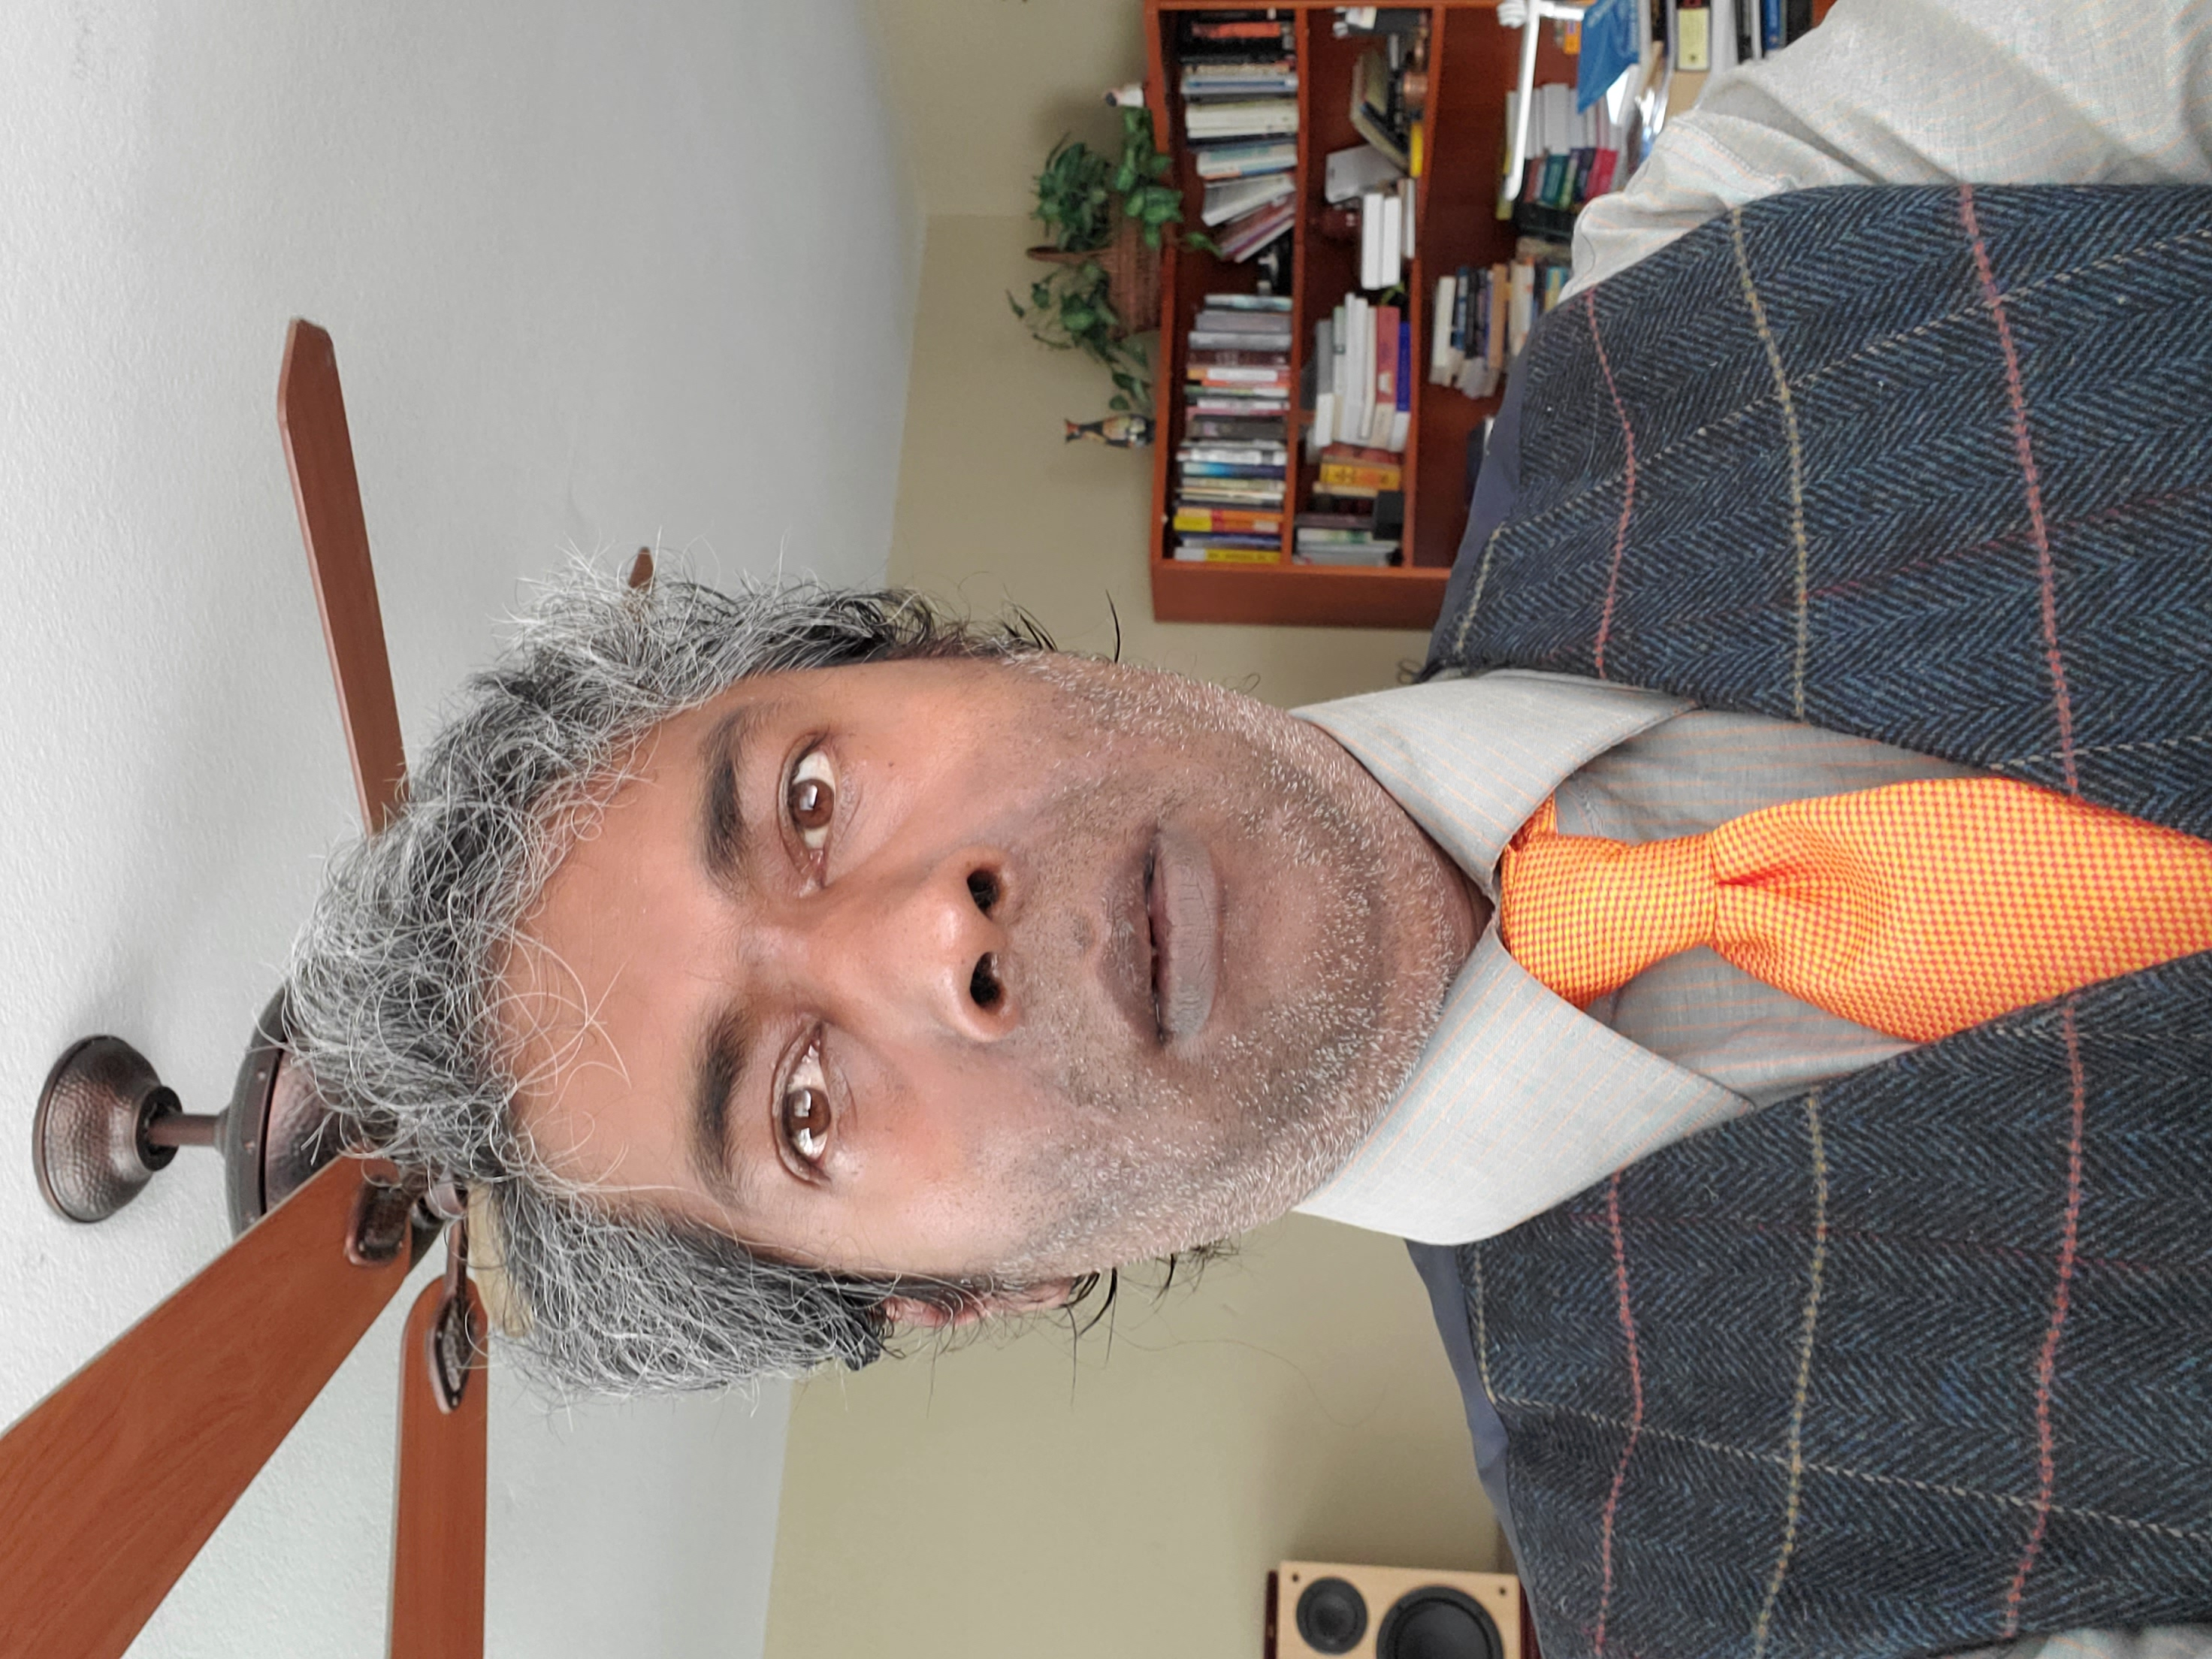
\includegraphics[angle=270,scale=0.16]{may19-2021.jpg}

After some years of search for Universal Noise Model for Nature I came to the realisation that O. Barndorff-Nielsen had found the correct answer in 1976.  In the past years, I have had tremendous success with precise fitting of Barndorff-Nielsen Distributions to World Value Surveys Data.  In the past week I was able to produce a model of Human Race Trust distributions using precise fits of Barndorff-Nielsen Distributions.


\section{Warning Signs of Failure of Gaussian Errors: 1818 Wilhelm Bessel}

Wilhelm Bessel did one detailed study in Astronomy in 1818 and noted that the errors were generally in line with Gaussian but with a slight tendency for larger errors than predicted.  This is not too long after 1805 work on least-squares and others establishing the normal distribution.  To me it is quite astounding that this only began to be quite annoying in the 1960s, a century and a half later.  Barndorff-Nielsen's Distribution is the correct solution to this entire sordid episode of considering normal distribution to be Nature's error density.  It never was, and we are today extremely clear that Barndorff-Nielsen Distribution ought to be considered the Nature's Error Density and all theory and practice of Science should change to accomodate this.

\end{document}
